\chapter{Methodology}\label{chap:method}
\section{Datasets} \label{sec:dataset}
In this study, we use two public datasets of human activity, to evaluate the impact of overlapping windows in a wide range of subjects, activities, and conditions. 

\subsection{Dataset 1} \label{sec:dataset1}
 As the first dataset, we use the dataset described in~\cite{banos2012benchmark}, one of the most complete public datasets for HAR in terms of the number of activities and subjects. The dataset consists of data collected from 17 subjects of diverse profiles while wearing 9 Xsens\footnote{\url{https://www.xsens.com}} inertial measurement units (IMU) on different parts of their body. Subjects performed 33 fitness activities (Table \ref{tab:Activites1}) ranging from warm up to fitness exercises in an out-of-lab environment. Each sensor provides tri-directional acceleration, gyroscope, and magnetic field measurements, as well as, orientation estimates in quaternion format (4D). Similar to prior work in~\cite{banos2014window}, acceleration data was used in our study. The dataset also provides data for three sensor displacement scenarios namely ``default", ``self-placement" and ``mutual-displacement" to compare the sensor anomalies, but as in~\cite{banos2014window}, only the data from the default scenario is used in our study. 

%  start of Table1
\begin{center}
\begin{table}

\begin{tabular}{|>{\centering}m{6cm}|>{\centering}m{0.98cm}|>{\centering}m{6.3cm}|>{\centering}p{0.98cm}|}
\hline 
Activity  & Label  & Activity  & Label\tabularnewline
\hline 
\hline 
No activity  & 0  & Upper trunk and lower body opposite twist (20x)  & 18\tabularnewline
\hline 
Walking (1 min)  & 1  & Arms lateral elevation (20x)  & 19\tabularnewline
\hline 
Jogging (1 min)  & 2  & Arms frontal elevation (20x)  & 20\tabularnewline
\hline 
Running (1 min)  & 3  & Frontal hand claps (20x)  & 21\tabularnewline
\hline 
Jump up (20x)  & 4  & Arms frontal crossing (20x)  & 22\tabularnewline
\hline 
Jump front \& back (20x)  & 5  & Shoulders high amplitude rotation (20x)  & 23\tabularnewline
\hline 
Jump sideways (20x)  & 6  & Shoulders low amplitude rotation (20x)  & 24\tabularnewline
\hline 
Jump leg/arms open/closed (20x)  & 7  & Arms inner rotation (20x)  & 25\tabularnewline
\hline 
Jump rope (20x)  & 8  & Knees (alternatively) to the breast (20x)  & 26\tabularnewline
\hline 
Trunk twist (arms outstretched) (20x)  & 9  & Heels (alternatively) to the backside (20x)  & 27\tabularnewline
\hline 
Trunk twist (elbows bended) (20x)  & 10  & Knees bending (crouching) (20x)  & 28\tabularnewline
\hline 
Waist bends forward (20x)  & 11  & Knees (alternatively) bend forward (20x)  & 29\tabularnewline
\hline 
Waist rotation (20x)  & 12  & Rotation on the knees (20x)  & 30\tabularnewline
\hline 
Waist bends 

(reach foot with opposite hand) (20x)  & 13  & Rowing (1 min)  & 31\tabularnewline
\hline 
Reach heels backwards (20x)  & 14  & Elliptic bike (1 min)  & 32\tabularnewline
\hline 
Lateral bend 

(10x to the left + 10x to the right)  & 15  & Cycling (1 min)  & 33\tabularnewline
\hline 
Lateral bend arm up

(10x to the left + 10x to the right)  & 16  & -  & -\tabularnewline
\hline 
Repetitive forward stretching (20x)  & 17  & -  & -\tabularnewline
\hline 
\end{tabular}

      % Title of the table
        \caption{Activity set in dataset 1.}        
        \label{tab:Activites1}
\end{table} 
\end{center}


\subsection{Dataset 2} \label{sec:dataset2}
The second dataset used is also one of the most complete and big public datasets for HAR in terms of the number of activities and subjects~\cite{morris2014recofit}. The dataset contains data for 74 activities (Table~\ref{tab:Activites2}) from 94 subjects (28 female), ages 18-58 ($\mu=34.2$). The data was collected in a large lab space from an armband worn on the right forearm, containing a SparkFun “Razor IMU” inertial sensor\footnote{\url{https://www.sparkfun.com}}. This IMU includes a 3-axis accelerometer and a 3-axis gyroscope ,which transmit sensor values to a PC at 50Hz. As can be seen in Table~\ref{tab:Activites2}, there are several activities in the dataset such as "Arm band adjustment" and "Device on Table" which we consider as noise in this study. Besides, since during the data collection, the subjects wore a single joint sensor on their right forearm, the activities of the opposite hand (left hand) can not be captured properly with the sensors. Thus, we have done a relabeling process to clarify the dataset. In this process, (1) we label all the irrelevant and opposite hand activities as a "Noise" class (2) all the activities that refer to multiple labels are grouped together as one exercise. Table~\ref{tab:Activites2} shows all the activities and their labels after the relabeling process.   

\begin{table}
\setlength\tabcolsep{1pt}
    \small
    \centering
%\footnotesize\setlength{\tabcolsep}{2.5pt}

\begin{tabular}{|c|c|c|c|c|c|}
\hline 
Activity & Label & Activity & Label & Activity & Label\tabularnewline
\hline 
Arm band adjustment & 1(Noise) & Lawnmower (both) & 20 & Squat (arms in front) & 33\tabularnewline
\hline 
Arm straight up & 1(Noise) & Lawnmower (left) & 1(Noise) & Squat (hands behind head) & 33\tabularnewline
\hline 
Band Pull-Down row & 2 & Lawnmower (right) & 21 & Squat (kettlebell) & 33\tabularnewline
\hline 
{}Bicep Curl & 3 & Lunge (both legs) & 22 & Squat Jump & 33\tabularnewline
\hline 
Bicep Curl (band) & 3 & Ball Slam & 23 & Squat Rack Shoulder Press & 33\tabularnewline
\hline 
Box Jump & 4 & No Exercise & 1(Noise) & Static Stretching & 1(Noise)\tabularnewline
\hline 
Burpee & 5 & Note & 1(Noise) & Stretching & 1(Noise)\tabularnewline
\hline 
Butterfly sit-up & 6 & {}Triceps Extension(standing) & 24 & Tap IMU & 1(Noise)\tabularnewline
\hline 
Chest Press & 7 & Triceps Extension (both) & 24 & Tap left IMU & 1(Noise)\tabularnewline
\hline 
Crunch & 8 & Plank & 25 & Tap right IMU & 1(Noise)\tabularnewline
\hline 
Device on Table & 1(Noise) & Power Boat pose & 26 & Triceps Kickback(bench --both) & 34\tabularnewline
\hline 
Dip & 9 & Pushups (foot variation) & 27 & Triceps Kickback (bench --left) & 1(Noise)\tabularnewline
\hline 
Dumbbell Deadlift Row & 10 & {}Pushups & 27 & Triceps Kickback (bench --right) & 34\tabularnewline
\hline 
{}Dumbbell Row (both) & 11 & Stretching & 1(Noise) & {}Triceps Extension (lying --both) & 35\tabularnewline
\hline 
Dumbbell Row (left) & 1(Noise) & Rest & 1(Noise) & Triceps Extension (lying --left) & 1(Noise)\tabularnewline
\hline 
Dumbbell Row (right) & 12 & Rowing Machine & 28 & Triceps Extension (lying --right) & 35\tabularnewline
\hline 
Dumbbell Squat (hands at side) & 13 & Running & 29 & Two-arm Dumbbell Curl (both) & 36\tabularnewline
\hline 
Dynamic Stretch & 1(Noise) & Russian Twist & 30 & Non-listed & 1(Noise)\tabularnewline
\hline 
Elliptical Machine & 14 & Seated Back Fly & 31 & V-up & 37\tabularnewline
\hline 
Punches & 15 & {}Shoulder Press & 32 & Walk & 38\tabularnewline
\hline 
Invalid & 1(Noise) & Side Plank (left) & 25 & Walking lunge & 39\tabularnewline
\hline 
Jump Rope & 16 & Side Plank (right) & 25 & Wall Ball & 40\tabularnewline
\hline 
Jumping Jacks & 17 & Sit-up (hand behind head) & 6 & Wall Squat & 41\tabularnewline
\hline 
Kettlebell Swing & 18 & Sit-up & 6 & Dumbbell Curl (alternating) & 36\tabularnewline
\hline 
{}Lateral Raise & 19 & Squat & 33 &  & \tabularnewline
\hline 
\end{tabular}
    \caption{Activity set in dataset 2.}
    \label{tab:Activites2}
\end{table}

\section{Experimental Setup} \label{sec:experiment setup}
Similar to prior work~\cite{banos2014window}, we did not apply any pre-processing to the dataset. We used both overlapping and non-overlapping windows. Overlapping windows were sliding at 200~ms, with window sizes ranging from 0.25~s to 7~s in steps of 0.25 s. For instance, a 5-second window shared 4.8~s of data with the previous one.  Given the constant value of the sliding duration (200 ms), using a set of different window sizes is equivalent to exploring the impact of various overlapping sizes on the performance of our HAR systems. For non-overlapping windows, we used the same settings as in~\cite{banos2014window}: disjoint windows with sizes ranging from 0.25~s to 7~s in steps of 0.25 s. We used the same feature sets as in~\cite{banos2014window}, namely FS1 (mean only), FS2 (mean and standard deviation) and FS3 (mean, standard deviation, maximum, minimum and mean crossing rate). Finally, for the classification part, we used the following classifiers: DT, KNN (K=3), NB and Nearest Centroid Classifier (NCC). We used these classifiers as implemented in scikit-learn 0.20~\cite{pedregosa2011scikit} with default hyperparameters. We have also investigated non-default hyperparameters in another experiment. Furthermore, to provide a comparison with the framework in~\cite{omid2019MPR}, we have utilized time-domain histogram features and the AdamOptimizer algorithm in Tensorflow 1.12.0 to train a neural network classifier with Sigmoid and Softmax trigger functions in the hidden and output layers, respectively. Such experiments will be explained in details in Chapter~\ref{chap:result}.
 
To evaluate model performance, we used both subject-dependent CV and subject-independent CV. We use the F1-score as a performance measure due to its robustness in class imbalance. F1-score which reaches its best at 1 and worse at 0, is computed as follows:
 \begin{center}
      $F1= \frac{2\times(precision \times recall)}{(precision + recall)}$
 \end{center}

All the source code for the conducted experiments are available in our GitHub repository \footnote{\url{http://www.github.com/big-data-lab-team/paper-generalizability-window-size}}. The repository contains the scripts to segment the datasets for different window sizes, feature sets and sliding window techniques. There is also a script for training and testing all mentioned classifiers on windowed datasets. Finally, it also contains code to reproduce all presented figures in this paper.

\subsection{Appendix} \label{sec:appendix}
In this section, the utilized classifiers in this study are explained.

\subsubsection{Decision Tree}
Decision Tree is a non-parametric supervised learning method used for classification and regression~\citep{duda2012pattern}. A decision tree is a tree-like or flowchart-like structure which is constituted of several nodes and branches. Nodes can be categorized into two types namely internal nodes (decision Node) which show a test on a feature of dataset and leaves (terminal Node) which represent a class label of the dataset. Regarding the branches, they basically represent the output of the test on internal nodes. A tree is constructed by splitting the training dataset into subsets based on a set of tests on the values of a certain feature. This process follows a recursive manner meaning that for each derived subset it is repeated. The recursion is finished when the classes of all samples in the subset at a node are the same or when partitioning the data does not improve the prediction. The primary challenge in the growing the decision tree (learning phase) is to select the best attribute as the root node and also each level to split the dataset. To do so, the impurity of each node should be calculated. Table~\ref{tab:dt_criterion} indicates the most widely used criterion for measuring the node impurity. Using such techniques, at each internal node, the entropy of all attributes in dataset are calculated and one with lowest entropy is selected to split the dataset. In scoring time for a give data point, we start from the root of the tree and apply its test on corresponding attribute of data point. On the basis of result, we follow the corresponding branch and jump to next level. We continue until we reach a leaf node which contains with predicted class value.   


\begin{table}[h]
    \centering
\begin{tabular}{|c|c|>{\centering}m{5cm}|}
\hline 
Criterion & Formula &Description \tabularnewline
\hline 
\hline 
Gini Index & $\sum_{i} p(i)(1-p(i))$ & p(i) is the probability
that an arbitrary
sample belongs to
class i.\tabularnewline
\hline 
Entropy & $-\sum_{i} p(i)~log~p(i)$ & p(i) is the relative frequency of class i\tabularnewline
\hline 
Towing rule & $\frac{p_{L} p_{R}}{4}(\sum_{i}|(p(i|t_L) - (p(i|t_R)|)^2$ & where L and R
refer to the left and right sides of a given split respectively, and 
$p(i|t)$ is the relative frequency of class i at node t \tabularnewline
\hline 
\end{tabular}
    \caption{The most common utilized techniques for splitting the dataset in DT~\citep{zambon2006effect} }
    \label{tab:dt_criterion}
\end{table}


\subsubsection{K-Nearest Neighbors} 
KNN is an instance-based supervised learning method used for classification and regression~\citep{cover1967nearest}. This method is also categorized as non-generalizing learning algorithms since it does not learn a general internal model from training dataset, but simply stores all of the data points. KNN is based on a neighborhood majority voting scheme and
assigns the new instance to the most common class amongst its K nearest neighbors. Table~\ref{tab:KNN_distances} describes several metrics to measure the similarity of two vectors which can be used to find the k nearest neighbors of a given instance. Regarding the number of neighbors (K), according to~\citep{doi:10.1002/9780470977811.ch8}, increasing it may (1) improve the performance of the classifier (2) reduce the effect of noise on the classification (3) makes the decision boundary less distinct. It should be noted that choosing too big value for k may result in performance drop since it can destroy the locality and as a result KNN uses the not neighbors to classify the coming data point. 


\begin{table}[h]
    \centering
\renewcommand{\arraystretch}{2.5}
\begin{tabular}{|c|>{\centering}m{4cm}|c|>{\centering}m{4cm}|}
\hline 
Distance Metric & Formula & Distance Metric & Formula  \tabularnewline
\hline 
\hline 
 Euclidean& $\sqrt{\sum_{i=1}^{n} {(x_i - y_i)}^{2}}$  & Standardized
Euclidean &  $\sqrt{\sum_{i=1}^{n} \frac{{(x_i - y_i)}^{2}}{{x_{i}}^2}}$ \tabularnewline
\hline 
 City Block & ${\sum_{i=1}^{n} {|x_i - y_i|}}$ & Minkowski & $\sqrt[p]{\sum_{i=1}^{n} {{|x_i - y_i|}}^{p}}$ \tabularnewline
\hline 
Chebychev & $\max_i \{|x_i - y_i|\}$  & Cosine & $\frac{x.y}{||x||||y||}$\tabularnewline
\hline 
\end{tabular}
\caption{Common used distance metrics in KNN - x and y are two vectors with equal length}
    \label{tab:KNN_distances}
\end{table}
\renewcommand{\arraystretch}{1}


\subsubsection{Naïve Bayes} 
NB~\citep{theodoridis1998pattern} is a supervised learning algorithm based on the Bayes theorem with the naive assumption of feature independence given the value of the class variable. The following equations show the NB formula:
\begin{equation}
    P(y|x_1,x_2,... , x_n) = \frac{p(y)\prod_{i=1}^{n}p(x_i|y)}{p(x_1,x_2,... , x_n)}
\end{equation}{}
Where y represents classes and $x_1$ to $x_n$ are feature vector. Since $p(x_1,x_2,... , x_n)$ is constant given the input, we can use the following classification rule: 
\begin{equation}
   \hat{y} = arg  max_{y}p(y) \prod_{i=1}^{n}p(x_i|y)
\end{equation}{}
In general, there are several types of NB classifiers such as Gaussian NB, Multinomial NB and Complement NB which mostly differ by the assumptions they make about the distribution of $p(x_i|y)$.
\subsubsection{Nearest Centroid Classifier}
NCC~\citep{tibshirani2003class} is a classification model which widely used in text classification~\citep{tan2008improved}, bioinformatics~\citep{levner2005feature} and medical domain~\citep{sharma2010improved}. This classifier calculates the centroid (mean) of each class in training set and assigns to the observation the class whose mean is closet to the observation. The following equations show the training and predicting phases of NCC:

\noindent{\textbf{Training:}} given labeled training samples $\{ ({\Vec{x}}, y_1), ({\Vec{x}}, y_2),..., ({\Vec{x}}, y_n) \}$ where $\Vec{x}$ is feature vector and $y_i$ is the class label $\in$ \mathbf{Y}, for each class the centroid is calculated as follows:
\begin{equation}
   \Vec{u}_l =  \frac{1}{c_l} \sum_{i\in{c_l}}\Vec{x_i}
\end{equation}{}
where $C_l$ is the set of indices of samples belonging to class l \in \mathbf{Y}.

\noindent{\textbf{Prediction:}} The assigned class ($\hat{y}$) to a given observation ,$\Vec{x}_i$ calculated as follow:
\begin{equation}
 \hat{y} = arg min_{l\inY} ||\Vec{u}_l - \vec{x}||
 \end{equation}{}

\subsubsection{Artificial Neural Network}
An Artificial Neural Network (ANN) is a systematic procedure of data processing inspired by the nervous system function in animals. It tries to reproduce the brain logical operation using a collection of neuron-like entities to perform processing of input data~\cite{cortina2010analysis}. The basic processing unit of an ANN is called perceptron which is an approximation to the biological neuron. It is a decision-making unit with several input connections and a single output as shown in Figure~\ref{fig:perceptron}. The
input neuron $p_i$ is weighted with a connection weight $w_i$  $w_i$. The perceptron sums the dot product of weights and inputs vectors, and adds a bias b. The obtained total value (n) will be
transformed by a function (f) to produce the output value. This process is summarized as:
\begin{equation}
    a= f(b+ \sum_{j=1}^{i}{w_j p_j})
\end{equation}{}


The function f which is called activation function or transfer function is used to introduce non-linear properties into the network. Tables~\ref{tab:activation_func} shows the most widely used activation functions. 


% transformation

\begin{figure}[h]
    \centering
    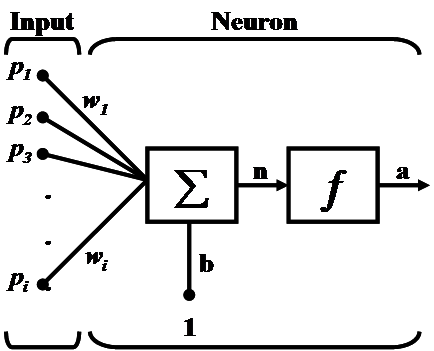
\includegraphics[width=.5\textwidth]{Figures/perceptron.png}
    \caption{Schematic representation of the perceptron extracted from~\cite{cortina2010analysis}.}
    \label{fig:perceptron}
\end{figure}



\begin{table}[h]
    \centering
\begin{tabular}{|c|c|}
\hline 
Activation function & Formula \tabularnewline
\hline 
Sigmoid & $f(x)= \frac{1}{1+ e^{-x}}$\tabularnewline
\hline 
Hyperbolic Tangent & $f(x)= \frac{1-e^{-2x}}{1+e^{-2x}}$\tabularnewline
\hline 
Rectified Linear units & $f(x)= max(x,0)$\tabularnewline
\hline 
\end{tabular}
    \caption{Commonly used activation functions in ANN}
    \label{tab:activation_func}
\end{table}



% It is a decision-making unit with several input connections and a single output, as shown in Figure 1. A signal p i which is delivered from an input i is multiplied on arrival by a connection weight w i , so that each signal appears at the perceptron as the weighted value w i p i . The perceptron sums the incoming signals and adds a bias b to give a total signal n. To this sum, a transfer function, usually a step-function, is applied to produce the output a. Inspired on its physiology, if the sum of inputs reaches the threshold level, the neuron is turned “on” and a message is sent out. If the sum is below the threshold value, the neuron is quiescent and remains “off”. This process is summarized in Equation 1.


